\section{Geometric Graph Generation with Chinese Restaurant Processes}
\label{sec: gggcrp}

The task of generative models is to learn from empirical observations how to model distributions and/or sample from them, and research into Generative Adversarial Networks (GANs) has yielded very successful solutions to the problem. Geometric graph generation is a way of representing graphs spatially, usually with node embeddings and assigning edges according to closeness w.r.t. a distance metric in embedding space. These techniques carry potential to transform a wide range of application domains, as with this approach, deep graph generative models are able to represent graphs in a more compact form. Research of this type is still ongoing to attempt to answer remaining questions posed by some experimental results. Namely, what is the best approach to further improve the scalability of the current state-of-the-art graph generation models, as the current best performance drops for larger graphs, while preserving their high expressive power and exchangeability?

In this section, we will present an approach to integrating permutation-invariant community-detection-based metrics into a Chinese Restaurant Process to perform exchangeable sequence modeling for graph generation. This approach, when integrated into the current-best graph GAN, yielded a new variation of the model, named GGG-CRP. Current results will be shown as comparable to the base model in the wake of strong resource reduction, demonstrating promise for improvement in immediate future work.

\subsection{Equivariant \& autoregressive}

The task of generative models is to learn from empirical observations how to
model distributions and/or sample from them. Research into Generative Adversarial Networks (GANs) has yielded very successful solutions to the problem, and results were already incredible and human-like with audio-visual data \cite{karras_analyzing_2020}. However, graphs are a challenging variant; they are \emph{discrete} structures with potential for highly complex relational structure. 
Earlier studies on GANs for graph generation (\cite{bojchevski_netgan_2018, de_cao_molgan_2018}) yielded models with relatively good performance, though they tended to memorize training data in the lack of domain-specific rewards or specific data properties. Therefore, to mitigate this issue of limited model applicability, more generalizable approaches started to gain popularity, such as geometric techniques.

\emph{Geometric} graph generation is a way of representing graphs spatially, usually with node embeddings and assigning edges according to closeness w.r.t. a distance metric in embedding space. With this approach, deep graph generative models represent graphs in a more manageable form and carry potential to transform a wide range of application domains: computational chemistry (novel drug discovery), electrical circuit modelling and design (complete automation of this process), computational biology (novel synthetic proteins), etc.

As noted by \cite{krawczuk_gg-gan_2020}, a graph generator $g$ should possess 4 desirable properties:
\begin{enumerate}[1.]
\item \emph{Expressive power} - $g$ should be able to model local and global dependencies between nodes and graph edges, going beyond simple degree statistics and learning structural features and motifs;
\item \emph{Scalability} - $g$ should have efficient computation, its tractability should be invariant to graph size;
\item \emph{Isomorphism consistency} - alike e.g., convolutional networks, $g$ should respect the permutation symmetry of its domain of graphs \cite{bronstein_geometric_2021}, i.e., assign isomorphic graphs the same probability, a property also referred to as exchangeability/permutation equivariance;
\item \emph{Novelty} - $g$ should produce non-isomorphic graphs that are similar to (but not necessarily in) the training set.
\end{enumerate}

To satisfy these properties, \cite{krawczuk_gg-gan_2020} proposed such an exchangeable geometric generator called GG-GAN. Surprisingly, classical geometric approaches have so far found limited adoption in the context of deep generative graph models. GG-GAN precisely bridges this gap, showing how deep geometric approaches can perform well. It sheds light on some basic limits and challenges of geometric graph generators and solves these problems with a novel latent state, while retaining consistency through equivariance.

This research is still ongoing, to attempt to answer remaining questions posed by some experiment results, namely: what is the best approach to further improve the scalability of the GG-GAN graph generation model, as the current best performance drops for larger graphs, while preserving its high expressive power and exchangeability. The work for this project consisted of focusing on the implementation of one of the proposed approaches: exchangeable sequence modeling with Chinese Restaurant Processes (CRPs), assisted by overlap-agnostic community detection, to incur the distribution modelling benefits of autoregressive models without sacrificing generation novelty and diversity. 

\subsection{Background}
\label{sec:background_gggcrp}

\subsubsection{Preliminaries}

\begin{definition}
    Given a set of samples $\mathcal{D}=\offf{\of{\mathbf{X}_i}}_{i=1}^{N}$, with $\mathbf{X}_i \in \mathbb{R}^F$, a \emph{generative model} $\mathcal{M}=\offf{f,g}$ models sample likelihoods as $\mathbb{P}\of{\mathbf{X} \in \mathcal{D}}=\sigma\of{f\of{\mathbf{X}}}$ with $f: \mathbb{R}^F \to \mathbb{R}$, and generates new samples from the dataset as $\hat{\mathbf{X}}=g\of{Z}$, from sampled latent noise $Z\in\mathbb{R}^D$ with $g_n:\mathbb{R}^D \to \mathbb{R}^F$. The optimal sampler $g$ is found most commonly by minimizing the expected \emph{negative log-likelihood loss}:
    \begin{equation}
        g^*=\argmin_{g}{\mathbb{E}_{\mathcal{D},Z}\off{-\log{\mathbb{P}\of{g\of{Z} \in \mathcal{D}}}}}=\argmin_{g}{\mathbb{E}_{\mathcal{D},Z}\off{-\log{\sigma\of{f\of{g\of{Z}}}}}}
    \end{equation}
\end{definition}

Wasserstein GANs are one of the most powerful generative models.

\begin{definition}
   A Wasserstein Generative Adversarial Network (WGAN) \cite{arjovsky_wasserstein_2017} is a generative model $\mathcal{M}=\offf{d,g}$, where both $d$ and $g$ are parametrized as neural networks whose parameters are optimized with min-max optimization of the \emph{Wasserstein distance}:
   \begin{equation}
   g^*=\argmin_{g}\max_{\text{1-Lipschitz } d}{\mathbb{E}_{\mathbf{X}\in\mathcal{D},Z}\off{d\of{\mathbf{X}}-d\of{g\of{Z}}}},
    \end{equation}
   where the primal variable $g$ is referred to as the \emph{generator} and the dual variable $d$ as the \emph{discriminator}. The 1-Lipschitz constraint for the dual variable is enforced artificially through various empirical techniques.
\end{definition}

\begin{definition}
Given the dataset $\mathcal{D}=\offf{\of{n_i,\mathbf{X}_i,A_i,\mathbf{y}_i}}_{i=1}^{N}$, where $n_i$ is the number of nodes in the $i$-th graph sample, $\mathbf{X}_i \in \mathbb{R}^{n_i \times F_V}$ is the matrix of node features, $A_i \in \offf{0,1,\dots,\abs{R}}^{n_i \times n_i}$ is the graph adjacency matrix enhanced with edge label information and $\mathbf{y}_i \in \mathbb{R}^{F_G}$ is the vector of global graph features, \emph{dense graph generation} involves learning a generative model $\mathcal{M}=\offf{f,g}$ for this specific sample structure. 

Formally, $\mathcal{M}$ samples graph sizes $n$, models the likelihood as $\mathbb{P}\of{\of{\mathbf{X},A,\mathbf{y}} \in \mathcal{D}}=\sigma\of{f_n\of{\mathbf{X},A,\mathbf{y}}}$ with $f_n: \mathbb{R}^{n \times F_V} \times \offf{0,1,\dots,\abs{R}}^{n \times n} \times \mathbb{R}^{F_G} \to \mathbb{R}$, and generates new samples from the dataset as $\of{\hat{\mathbf{X}},\hat{A},\hat{\mathbf{y}}}=g_n\of{Z}$, from latent noise $Z\in\mathbb{R}^D$ with $g_n:\mathbb{R}^D \to \mathbb{R}^{n \times F_V} \times \offf{0,1,\dots,\abs{R}}^{n \times n} \times \mathbb{R}^{F_G}$.
\end{definition}

\subsubsection{Geometric Graph Generation with GG-GAN}
Two main issues plague current top non-equivariant graph generators: 
\begin{itemize}
\item Even though they can approximate any distribution arbitrarily up to their constraints, they can \emph{waste a significant portion of capacity} modeling graphs that are isomorphic to each other - the isomorphism consistency property guaranteed by models like GG-GAN is a solution;
\item In general, they are not \emph{injective} functions; they have no guarantee that two random latent vectors will not be mapped to the same graph (\emph{collisions}) - GG-GAN's novel generator latent state helps to mitigate this problem, though not yet completely.  
\end{itemize}

GG-GAN \cite{krawczuk_gg-gan_2020} is an LP-penalty Wasserstein GAN \cite{gulrajani_improved_2017} with a permutation-equivariant generator and discriminator duo. GG-GAN's generator $g$ conceptually consists of three serially-connected parts; its architecture is visually represented in Figure \ref{fig:gg_gan_g}. The \emph{root} constructs the node latent state used as initialization from the generator. Here the novel alternative to the standard Gaussian latent state, $Z_i \in \mathbb{R}^{n_i \times D} \sim N\of{0,\mathbf{I}}$, is the idea to leave $P<D$ of the latent dimensions as \emph{fixed}, while the remaining a part of a single random context vector $z \in \mathbb{R}^{D-P}$. This fixed point set $\Phi_i \in \mathbb{R}^{n_i \times P}$ could either be a fully-learnable parameter set or, e.g., chosen fixed points in a higher-dimensional binary or spherical embedding space. With this setup, the collision avoidance task is addressed together with the instability issues of GAN training at the same time. 

The \emph{trunk} is a permutation-equivariant function $t: \mathbb{R}^D \to \mathbb{R}^{F}$ that computes a further embedding of the node set, $X_i \in \mathbb{R}^{n_i \times F}$, which is given to the \emph{edge readout} function $r: \mathbb{R}^{n_i \times F} \to \mathbb{R}^{n_i \times n_i}$ to transform it into a probabilistic adjacency matrix. The final adjacency output $A_i$ is obtained by sampling the sigmoid-activated readout values as Bernoulli random variables. A \emph{node readout} function with a similar structure can generate node features $\mathbf{X}_i$ if required. To guarantee equivariance, both the trunk and readouts utilize provably-equivariant deep layers such as (multi-head) attention or point-wise MLPs. To allow the generator \emph{adaptability} to variable graph sizes $n_i$, this single graph meta-variable is modeled and sampled as a categorical random variable whose probability mass function and range are estimated from the dataset.

The discriminator $d$, represented in Figure \ref{fig:gg_gan_d}, passes each graph input to two heads, whose output features are concatenated before a MLP classifier: one is a known permutation-equivariant Message Passing Neural Network (MPNN) from previous work, while the other computes classical handcrafted graph features in a differentiable manner - to preserve both universality and exchangeability of the discriminator.

\begin{figure}
    \centering
    \begin{minipage}{0.475\textwidth}
    \centering
    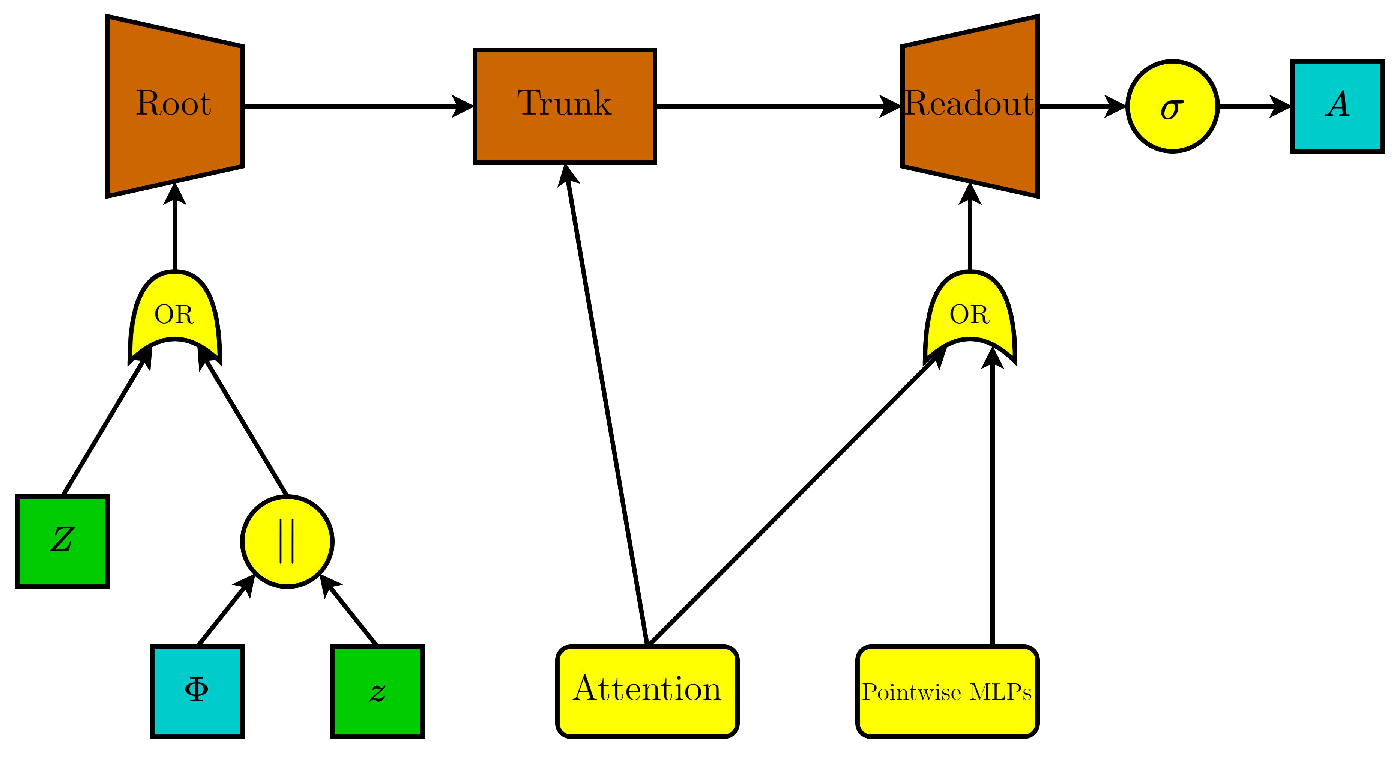
\includegraphics[width=\textwidth]{figures/gggcrp/gg_gan_g.pdf}
    \caption{GG-GAN generator architecture.}
    \label{fig:gg_gan_g}    
    \end{minipage}
    \hfill
    \begin{minipage}{0.475\textwidth}
    \centering
    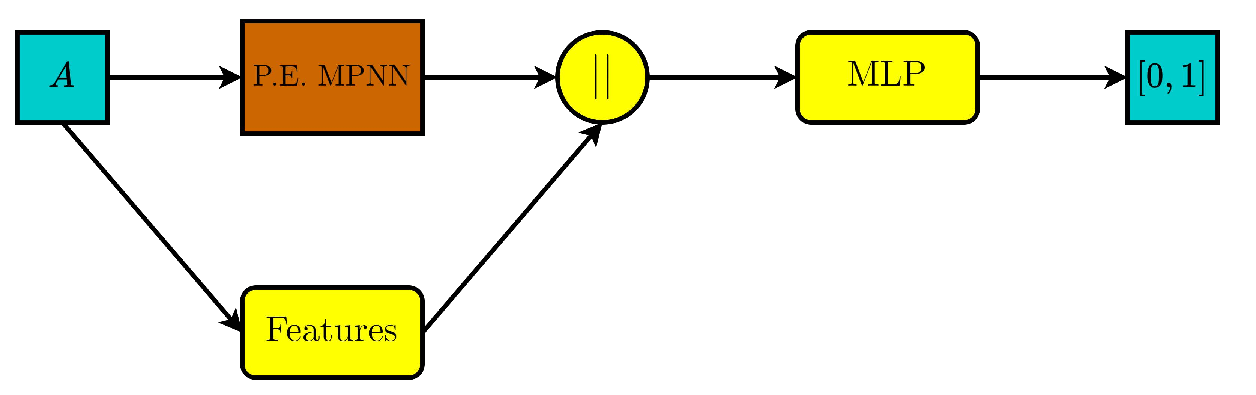
\includegraphics[width=\textwidth]{figures/gggcrp/gg_gan_d.pdf}
    \caption{GG-GAN discriminator architecture.}
    \label{fig:gg_gan_d}    
    \end{minipage}
\end{figure}

\subsubsection{Chinese Restaurant Processes}
In probability theory, the Chinese Restaurant Process (CRP) is a discrete-time stochastic process, analogous to a customer-table assignment sequence in a restaurant \cite{aldous_exchangeability_1985}. Imagine a restaurant with an infinite number of circular tables, each with infinite capacity. Each customer chooses to either sit at an occupied table with a probability proportional to the number of customers already there or at an unoccupied table. At time $n$, $n$ customers have been partitioned among $k \leq n$ tables (or \emph{blocks} of the partition).

\begin{definition}
    Formally, given $n \in \mathbb{N}$, at time $n$ the \emph{Chinese Restaurant Process} is the collection of random variables $\pmb{X}=\offf{X_i}_{i=1}^{n}$ whose support is $\mathcal{P}_n$, the set of all integer partitions of the number $n$, i.e. $\sum_{i=1}^{n}{X_i}=n$. The CRP's probability transition function is given by: 
\begin{equation}
\mathbb{P}\of{\pmb{X}=\offf{x_i}_{i=1}^{n} \vert \pmb{X}=\offf{y_i}_{i=1}^{n-1}}
= \begin{cases} 
\frac{y_k}{n}, & x_n=0, x_k = y_k+1 \wedge \forall j \neq k, x_j=y_j \\
\frac{1}{n}, & x_n = 1 \wedge \forall j \leq n-1, x_j=y_j \\
0, & \text{otherwise} \end{cases}
\end{equation}
\end{definition}

Based on this and using the ratio definition and chain rule of probability, it can be shown that the CRP's probability mass function can be given by: 
\begin{equation}
\mathbb{P}\of{\pmb{X}=\offf{x_i}_{i=1}^{n}} = \frac{1}{n!}\prod_{i=1}^{n}{\of{x_i - 1}!}
\end{equation}
So we observe the main benefit of the CRP, the realizations of this process are exchangeable, meaning the order in which the \enquote{customers sit} does not affect the probability of the final distribution, as due to the permutation-invariance of products, it only depends on the block size values and not their order. This is a very useful property, as it leads to the possibility of building an autoregressive variant of the GG-GAN generator that will remain exchangeable, by envisioning graph nodes as the \enquote{customers} and generalizing the CRP block (\enquote{table}) assignment to be agnostic to graph structure (instead of purely stochastic).

\subsubsection{Overlapping Community Detection}
Both historic and more recent overview studies (\cite{xie_overlapping_2013, li_deeper_2018, liu_deep_2020, vieira_comparative_2020}) suggest that matrix factorization, heuristic, and deep model approaches all exhibit satisfactory overlapping community detection performance. These studies evaluate the different methods on known benchmark datasets for overlapping community detection, such as the LFR benchmark \cite{lancichinetti_benchmarks_2009} and dedicated appropriate scoring metrics.

Research into deep Graph Neural Network (GNN) overlapping community classifiers is known to be very limited, but the few published models already display excellent results \cite{jia_communitygan_2019, wang_unifying_2020}. However, their main downside is that they are classification models that need to be pre-trained with at least some known community labels for the dataset, i.e., all are semi-supervised approaches. In addition, recently \cite{huang_combining_2020} has pointed out that due to their message passing nature, community detection GNNs are not unlike the classic label propagation algorithm in terms of distributing and assigning labels, in this case, community membership, to nodes. Indeed, they show that with certain techniques, label propagation can achieve comparable results to GNNs.

The state-of-the-art algorithm for disjoint community detection remains the Leiden algorithm \cite{traag_louvain_2019}, as we discussed previously as well. An heuristic-based approach, it is an improvement of the classic Louvain algorithm. It provides very useful guarantees that Louvain was discovered to not: no detected community is formed from more than one connected component, and itself is not a disconnected component of the full graph. It has been proven to be the current best due to these properties and its excellent scalability to very large graphs. For overlap-agnostic heuristic algorithms, many proven options exist: EgoNetSplitter \cite{epasto_ego-splitting_2017}, LEMON \cite{li_local_2018}, LPANNI \cite{lu_lpanni_2019}, CPPR \cite{gao_overlapping_2021}, etc. The benefits of heuristic-based algorithms are their high efficiency and direct output of the communities, though detection accuracy is not always guaranteed.

Matrix factorization methods usually display higher accuracy and always support overlaps, though they suffer from higher computation costs, and since the partitioning is most often represented as a real-valued matrix, discretization is usually required to obtain the community membership. Best-performing models of this type are BigClam \cite{yang_overlapping_2013}, MNMF \cite{wang_community_2017}, DANMF \cite{ye_deep_2018}. To perform the discretization required for the output of these models, one can, e.g., employ the background edge probability threshold proposed in \cite{jia_communitygan_2019}. An interesting case is the DNMF method by \cite{ye_discrete_2019}, as it solves an additional optimization problem to find the optimal discretization of the original decomposed matrix output, therefore not requiring introduction of implicit bias through a separate discretization, though by doing so, incurring higher computational cost.

Interestingly, some authors have successfully employed reinforcement learning for this task. \cite{zhang_mixed_2017} and \cite{bello-orgaz_multi-objective_2018} have developed evolutionary algorithms for overlapping community detection, while \cite{wang_effective_2021} instead formulated the problem in a game theory setting. 

As hinted in the previous section, we require a CRP block assignment that will be agnostic to graph structure. As (overlapping) communities represent a natural \enquote{ground-truth} partitioning of a graph, we believe they are the most appropriate to be used as CRP blocks. After careful consideration of their properties and code availability, it was decided to validate only most of the heuristic- and matrix-factorization-based algorithms for this project. Credit to \cite{csardi_igraph_2006, rozemberczki_karate_2020, li_local_2018, janchevski_dnmf-python_2022} for the implementations.

\subsection{Methodology}
\label{sec:methodology_gggcrp}

In the following text, we will present our approach on how to integrate permutation-invariant community-based metrics into a CRP to perform exchangeable sequence modelling for graph generation. This approach, when integrated into GG-GAN, yields a new variation of the model, tentatively named GGG-CRP. 

\textbf{Notes on notation:} $\mathbb{N}_{m} = \offf{1,\dots,m}$ will denote the set of the first $m$ natural numbers; the index $i$ will denote a batch sample (graph); $j$ will denote the \emph{cardinality} of an overlapping region, defined as the number of different communities that are overlapping to form the region; $k$ will denote a community and $l$ will denote a single node.

\subsubsection{Data augmentation}
The first step required for the new graph distribution modeling approach for GG-GAN is to run a selected overlapping community detection algorithm on each graph in the dataset. The dataset for GG-GAN is represented as the set $\mathcal{D} = \offf{\of{\mathbf{X}_i, A_i}}_{i=1}^{N}$, where $\mathbf{X}_i$ are the node feature vectors, $A_i$ are the graph adjacency matrices, i.e., we do not consider global graph features. We condense and represent the output of the graph partitioning algorithm through the matrix $M_i = \text{OCD}\of{A_i} \in \offf{0, 1}^{n_i \times k_i}$, which from here on shall be referred to as the \emph{membership matrix}. $k_i \leq n_i$ is the number of detected communities and $M_{i,l,k}=1$ denotes that in graph $i$, node $l$ is a member of community $k$.

The membership matrix in the general case has two natural constraints: all communities must be non-empty, $\forall k \in \mathbb{N}_{k_i}, \of{M^T_i \cdot \mathbf{1}_{n_i}}_k > 0$; all nodes must be assigned $\forall l \in \mathbb{N}_{n_i}, \of{M_i \cdot \mathbf{1}_{k_i}}_l > 0$. In the special case of disjoint communities, this property is represented by $M_i$ satisfying additionally: $M_i \cdot \mathbf{1}_{k_i} = \mathbf{1}_{n_i}$.

During model training, as will also be evident from later explanations, the new generator would require only the membership matrix as additional input from the data. However, for graph sampling during evaluation, novel node permutation-invariant graph meta-statistics are required as a replacement for it. One is the \emph{overlapping region size matrix} $O_i \in \of{\mathbb{N}\cup\offf{0}}^{k_i \times k_i}$, where $O_{i,j,k}$ counts how many nodes of overlapping region cardinality $j$ are members of community $k$ for graph $i$. It can be computed directly from the membership matrix:
\begin{equation}
O_i = \text{OneHotEncode}\of{M_i \cdot \mathbf{1}_{k_i}}^T \cdot M_i
\end{equation}
The \emph{community size vector} $c_i \in \mathbb{N}^{k_i}$ counting the number of nodes assigned to each community can also easily be computed: 
\begin{equation}
c_i = M^T_i \cdot \mathbf{1}_{n_i} = O_i^T \cdot \mathbf{1}_{k_i}
\end{equation}
In the special case of disjoint communities, we have only cardinality-1 nodes (each nodes belongs to only one community): $O_{i,1}=c_i, O_{i,2}=\dots=O_{i,k_i}=\mathbf{0}_{k_i}$.
The final augmented dataset is thus the collection: $\mathcal{D}^* = \offf{\of{\mathbf{X}_i, A_i, k_i, c_i, O_i, M_i}}_{i=1}^{B}$.

\subsubsection{Modeling and sampling of permutation-invariant graph meta-variables}
Recall that in order for GG-GAN's generator to be robust to variation in graph size in a dataset, the graph size is estimated and sampled as a categorical random variable. We can now naturally improve the adaptability of the model by estimating and sampling the newly available community-related statistics as well.

\paragraph{Estimated distribution}
Instead of just the maximum graph size, the full list of estimated order statistics is now:
\begin{itemize}
\item Maximum graph size: $n_{\max}=\max_{i=1}^{N}{n_i}$
\item Maximum number of communities: $k_{\max}=\max_{i=1}^{N}{k_i}$
\item Maximum community size: $c_{\max}=\max_{i=1}^{N}\max_{k=1}^{k_i}{c_{i,k}}$
\item Maximum overlapping region size: $o_{\max}=\max_{i=1}^{N}\max_{j=1}^{k_i}\max_{k=1}^{k_i}{O_{i,j,k}}$
\end{itemize}

The full list of random variables and vectors that need to be modeled and sampled for GGG-CRP is:

\begin{itemize}
\item Number of nodes / graph size: $n \in \mathbb{N}_{n_{\max}}$
\item Number of overlapping region cardinalities: $K^c \in \mathbb{N}_{k_{\max}}$
\item Number of nodes per cardinality: $N^c \in \of{\mathbb{N}_{n_{\max}} \cup \offf{0}}^{k_{\max}}$
\item Number of communities per cardinality: $K \in \mathbb{N}_{k_{\max}}^{k_{\max}}$
\item Overlapping region size: $O \in \of{\mathbb{N}_{o_{\max}} \cup \offf{0}}^{k_{\max} \times k_{\max}}$
\end{itemize}

The collection of graph meta-variables is thus $\of{N, K^c, N^c, K, O}$ and to generalize GG-GAN's approach, is modeled with a jointly-categorical distribution $\mathcal{F}$ whose probabilities are estimated from the data as relative frequencies. In this manner, no independence assumptions are introduced, though for larger graphs, due to potential memory issues, a sparse implementation of the estimated probability tensors is recommended.

\paragraph{Graph meta-variable sampling}

The pseudocode of the full meta-variable sampling algorithm for GGG-CRP is given in Algorithm \ref{algorithm:graph_meta_sampling}. Note: a subscripted $\mathcal{F}$ in the pseudocode denotes a marginalized version of the joint meta-variable distribution.
\begin{algorithm}[H]
\caption{Graph meta-variable sampling}
\label{algorithm:graph_meta_sampling}
\begin{algorithmic}
\STATE{\textbf{sample} number of nodes and cardinalities: $n_i, K^c_i \sim \hat{\mathcal{F}}_{N,K^c}$}
\STATE{\textbf{sample} partition of nodes across cardinalities: $N^c_i \sim \text{PartitionDistribution}\of{n_i, K^c_i, \hat{\mathcal{F}}_{n_i, K^c_i, N^c}}$}
\FOR{cardinality $j \gets 1$ to $k_{\max}$}
\STATE{\textbf{sample} number of communities for cardinality: $K_{i,j} \sim \hat{\mathcal{F}}_{n_i, K^c_i, N^c_{i,j}, K_j}$}
\STATE{\textbf{sample} overlap region sizes: $O_{i,j} \sim \text{PartitionDistribution}\of{j \cdot N^c_{i,j}, K_{i,j}, \hat{\mathcal{F}}_{n_i, K^c_i, N^c_{i,j}, K_{i,j}, O_j}}$}
\STATE{\textbf{assign} nodes with cardinality: $\mathcal{N}_{i,j} \gets \offf{\sum_{k=1}^{j-1}{N^c_{i,k}},\dots,\sum_{k=1}^{j}{N^c_{i,k}}} \subseteq \mathbb{N}_{n_{\max}}$}
\STATE{\textbf{sample} membership: $M_{i,\mathcal{N}_{i,j}} \sim \text{BipartiteGraphDistribution}\of{j \cdot 1_{N^c_{i,j}},O_{i,j}}$}
\ENDFOR
\STATE{\textbf{compute} number of communities: $K_i \gets \max_{j=1}^{k_{\max}}{K_{i, j}}$}
\STATE{\textbf{compute} community sizes: $c_i \gets O^T_i \cdot 1_{k_{\max}}$}
\RETURN{$n_i, K_i, c_i, O_i, M_i$}
\end{algorithmic}
\end{algorithm} 

$\text{PartitionDistribution}\of{n,m,p}$ denotes the distribution over partitions of the integer $n$ into exactly $m$ parts, where $p$ is a probability distribution over the possible sizes of the parts in $\mathbb{N}_{n}$. Fristedt in \cite{fristedt_structure_1993} gives an algorithm that performs partition sampling, with the guarantee of the least amount of rejections and $\text{PartitionDistribution}\of{n,m,\text{Uniform}} \sim \text{Uniform}$, i.e., it is also provably unbiased in the case of uniform part size probabilities. 

Unfortunately, in the general scenario for our model, $p$ is not uniform if we wish to be robust to any region size distribution. Therefore, instead of this algorithm, we employed general rejection sampling. Further work might show how to extend Fristedt's guarantees to general part size distributions.
    
$\text{BipartiteGraphDistribution}\of{a,b}$ denotes the uniform distribution over all bipartite graphs with the two degree sequences $a$ and $b$. We can observe that each node-chunk membership matrix indeed can be viewed as a bipartite graph, where the other graph meta-variables represent its node and chunk degree sequences. The membership matrix of each graph has to be randomly sampled, as there are usually multiple valid solutions to the assignment problem. 
    
To sample a uniform random bipartite graph with degree constraints, one can employ methods such as the Configuration Model \cite{newman_structure_2003} or the Havel-Hakimi algorithm \cite{hakimi_realizability_1963, kleitman_algorithms_1973}. Another idea is to sample the assignment based on node-chunk distance in the root latent space. Formally, if the root's fixed latent point set is $\Phi_i \in \mathbb{R}^{n_i \times P}$, we can also assign a fixed latent representation for each community: $\Phi^c_i \in \mathbb{R}^{k_i \times P}$. If $\ell: \mathbb{R}^{P} \times \mathbb{R}^{P} \to \mathbb{R}$ is an appropriate distance metric for the latent space, then the assignment probabilities can be computed as: 
\begin{equation}
\mathbb{P}\of{M_{i,l,k}=1}=\frac{\ell\of{\Phi_{i,l},\Phi^c_{i,k}}}{\sum_{k' \in \mathbb{N}_{k_{\max}}}{\ell\of{\Phi_{i,l},\Phi^c_{i,k'}}}}
\end{equation}

\subsubsection{Exchangeable graph generation agnostic to community structure}
As stated above, to utilize the benefits of exchangeable autoregressive models, instead of single-shot graph generation, we will employ a block-by-block CRP-inspired technique. The generation will thus take place in multiple \emph{rounds}, such that in each round the edges incident to the nodes in one block will be generated. In this manner, the generated graph sequentially grows to its target size.

The first crucial decision is thus how to perform the block assignment of nodes, and as also stated above, the computed overlapping communities will serve the role of CRP blocks. Formally, given graph meta-data $\of{n_i, K_i, c_i, O_i, M_i}$, computed from the dataset or sampled, we compute the community sets $C_{i,1},\dots,C_{i,K_i} \subseteq \mathbb{N}_{n_i}$ according to the given membership matrix: 
\begin{equation}
\forall k \in \mathbb{N}_{K_i},C_{i,k}=\offf{l \in \mathbb{N}_{n_i} \mid M_{i,l,k} = 1}
\end{equation}
GGG-CRP's generator now computes the root for each block/round separately, by collecting the latent points according to the block assignment:
\begin{equation}
\forall k \in \mathbb{N}_{k_{\max}}, \forall l \in \mathbb{N}_{c_{\max}},
R_{i,l}^{\of{k}} = \begin{cases} z_i||\Phi_{i,C_{i,k,l}}, & l \leq c_{i,k} \\ 0, & \text{otherwise} \end{cases}
\end{equation}
The autoregressive architecture of GGG-CRP is facilitated through a new edge readout function $r'$, modified to accept the discriminator features of the current graph in addition to the trunk's output for the current block. 

With this setup in mind, GGG-CRP's generator pipeline design is given in Algorithm \ref{algorithm:crp_generator}. The main scalability benefits of autoregressive generation techniques for graphs lie in the reduction in memory complexity, as with this setup, only one CRP block of a graph is processed at a time.

\begin{algorithm}%[H]
\caption{GGG-CRP graph generation}
\label{algorithm:crp_generator}
\begin{algorithmic}
\STATE{\textbf{initialize} first graph: $A_{i}^{\of{1}} \gets r\of{t\of{R_{i}^{\of{1}}}}$}
\STATE{\textbf{initialize} prior: $\hat{\mathbf{X}}_{i}^{\of{1}} \gets R_{i}^{\of{1}}$}
\FOR{round $k \gets 2$ to $k_{\max}$}
\STATE{\textbf{update} graph: $A_{i}^{\of{k}} \gets r'\of{t\of{R_{i}^{\of{k}}},\hat{\mathbf{X}}_{i}^{\of{k-1}}}$}
\STATE{\textbf{update} prior: $\hat{\mathbf{X}}_{i}^{\of{k}} \gets d_f\of{A_{i}^{\of{k}}}$}
\ENDFOR
\RETURN{final generated graph $A_i = A_{i}^{\of{k_{\max}}}$}
\end{algorithmic}
\end{algorithm} 

Regarding scaling up performance to larger graphs, observe that if there were overlapping nodes present, each would have been added in the generated graph with exactly as many copies as its number of communities. This is intentional and we believe natural, as nodes belonging to multiple communities should have their representation refined multiple times as well. Due to this decision, however, all but the last-added copy of these nodes needs to be pruned from the final readout output, as well as the non-trailing zero-padding entries.

In addition, to mitigate a discovered vanishing gradient issue with the CRP generator (expected due to the now recurrent architecture), a BatchNorm layer was added after the trunk output in each round, and the readout attention layers were configured to use ReLU activation instead of Softmax.

\subsubsection{Multi-level connectivity regularization}
With the computation of community-based metadata for the graphs, we obtain a unique opportunity to add a special type of regularization for the generator. Namely, one can compute a coarsening of each graph, the connectivity between communities as nodes themselves. The generator would be evaluated now with an additional Wasserstein score added to the discriminator loss, computed based on this higher-level connectivity, with a dedicated regularization parameter. 

Formally, let $\of{\mathbf{X}_i, A_i, k_i, c_i, O_i, M_i}$ be a graph sample from the augmented dataset or sampled from the generator. One can compute the community-level features $\mathbf{X}^C_i \in \mathbb{R}^{k_i \times F}$ and (multiplex) edges $A^C_i \in \of{\mathbb{N} \cup \offf{0}}^{k_i \times k_i}$ in the following manner: 
\begin{equation}
\mathbf{X}^C_i = \of{M^T_i \cdot \mathbf{X}_i} \oslash c_i, A^C_i = M^T_i \cdot A_i \cdot M_i    
\end{equation}
The coarser graph sample is thus the collection $\of{\mathbf{X}^C_i, A^c_i, k_i}$.

We stress that the proper validation of this score's regularization parameter is crucial, since if the discriminator weighs too strongly the coarser connectivity, it will underfit as the coarse-to-fine graph mapping is not injective, leaving the generator a chance to fool the discriminator. This can also be mitigated by enriching the coarse graph with further features as edge weights, to reduce collisions.

\subsubsection{Experiments}

To preserve the relevance of comparisons, the experimental setup for evaluating GGG-CRP was planned as identical to the one for the original GG-GAN.

The list of datasets chosen for evaluation consisted of: the QM9 dataset \cite{de_cao_molgan_2018}, the HouseFloorplan dataset \cite{nauata_house-gan_2020}, the Chordal9 dataset \cite{mckay_chordal_2020}, and the Community20 dataset \cite{niu_permutation_2020}.

Expressive power was evaluated by comparing real and generated graphs w.r.t. 5 desired graph metrics of increasing complexity: node degree distribution, clustering coefficient, cycle distribution, algebraic connectivity, and degree assortativity. The comparison was performed through the Maximum Mean Discrepancy (MMD) scores of \cite{you_graphrnn_2018} computed between the generated and real metric distributions.

Generation novelty was evaluated by studying the number of different isomorphism classes generated, only considering those that differ from those in the training set.

\subsection{Results \& Discussion}
\label{sec:results_gggcrp}

Table \ref{tab:expressive_power} contains the MMD scores obtained by the current best-performing model configurations of each type. Unfortunately, we observe that even though GGG-CRP currently, for most metrics, can provide a comparable performance to GG-GAN for each dataset, a select few graph features prove difficult to train. A special case is perhaps the HouseFloorplan dataset, for which we obtain impressive performance with GGG-CRP, while GG-GAN could not scale to it at all.

\begin{table}[ht!]
\centering
\caption[Comparison of expressive power between GG-GAN and GGG-CRP.]{Comparison of expressive power between GG-GAN and GGG-CRP. Left to right: MMD values for distributions of degrees, clustering coefficients, cycle counts, algebraic connectivity, and degree assortativity. Lower MMD scores denote better performance.}
\label{tab:expressive_power}
% \setlength{\arrayrulewidth}{0.5mm}
% \adjustbox{width=\textwidth}{
\begin{tabular}{llrrrrr}
\toprule
Dataset & Model & Degree & Cluster & Cycle & AC & DA \\
\midrule
QM9 & GG-GAN & 0.0038 & 0.0341 & 0.0248 & 0.0206 & 0.0252 \\
QM9 & GGG-CRP & 0.1079  & 0.0234 & 0.2587 & 0.9121 & 0.0896 \\
Community20 & GG-GAN & 0.0023 & 0.4359 & 6.7E-6 & 0.0785 & 0.1312 \\
Community20 & GGG-CRP & 0.0110 & 0.4061 & 1.4186E-5 & 0.0861 & 0.4718 \\
Chordal9 & GG-GAN & 0.0281 & 0.0130 & 0.0455 & 0.0322 & 0.0690 \\
Chordal9 & GGG-CRP & 0.0203 & 0.0360 & 0.0092 & 0.9223 & 0.0733 \\
HouseFloorplan & GG-GAN & \textemdash & \textemdash & \textemdash & \textemdash & \textemdash \\
HouseFloorplan & GGG-CRP & 0.0033 & 0.0369 & 0.0129 & 7.3910E-6 & 0.0204 \\
\bottomrule
\end{tabular}
%}
\end{table}

We observe this visually as well: Figures \labelcref{fig:qm9,fig:community_20,fig:chordal9,fig:house} present visualizations of a set of sampled graphs from the CRP generator, as well as the real and fake degree and cycle distributions for each dataset. We observe that the HouseFloorplan distribution is learned well; however, a persistent lack of a few connecting edges can be observed for the other three datasets.

\begin{figure}[!ht]
    \centering
    \begin{minipage}{0.475\textwidth}
    \centering
    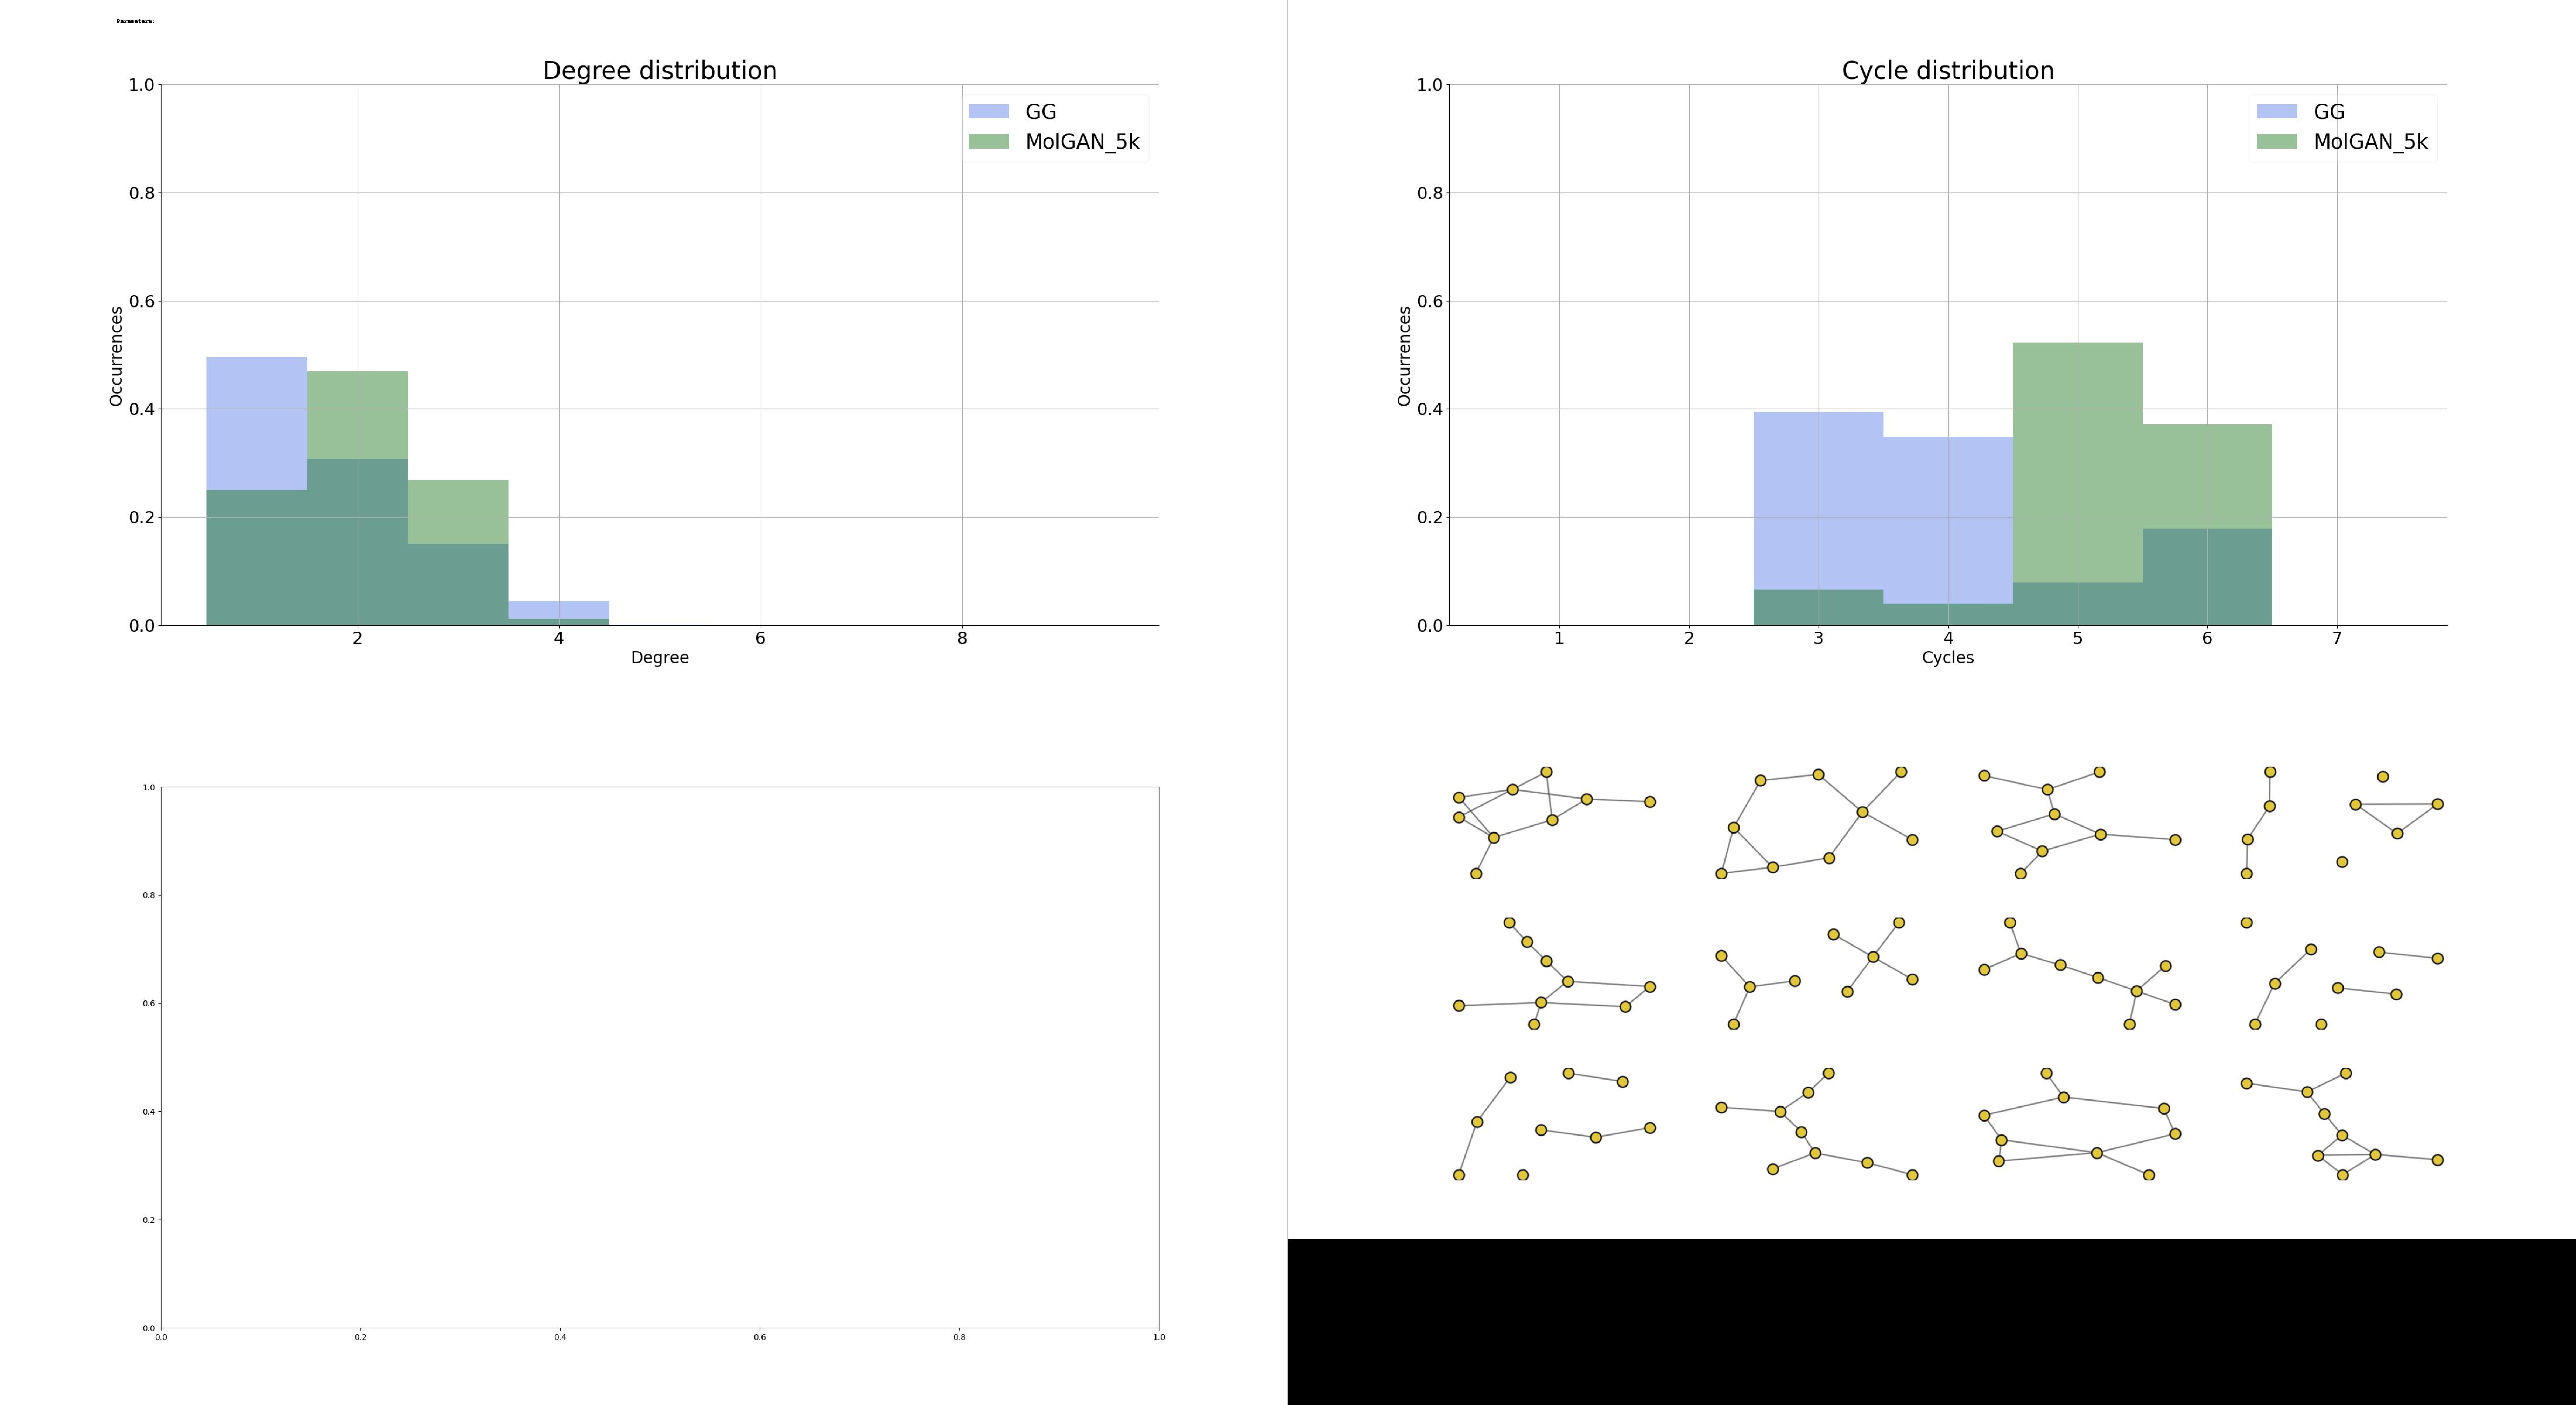
\includegraphics[width=\textwidth]{figures/gggcrp/QM9.pdf}
    \caption[GGG-CRP performance on QM9.]{QM9 performance.}
    \label{fig:qm9}    
    \end{minipage}
    \hfill
    \begin{minipage}{0.475\textwidth}
    \centering
    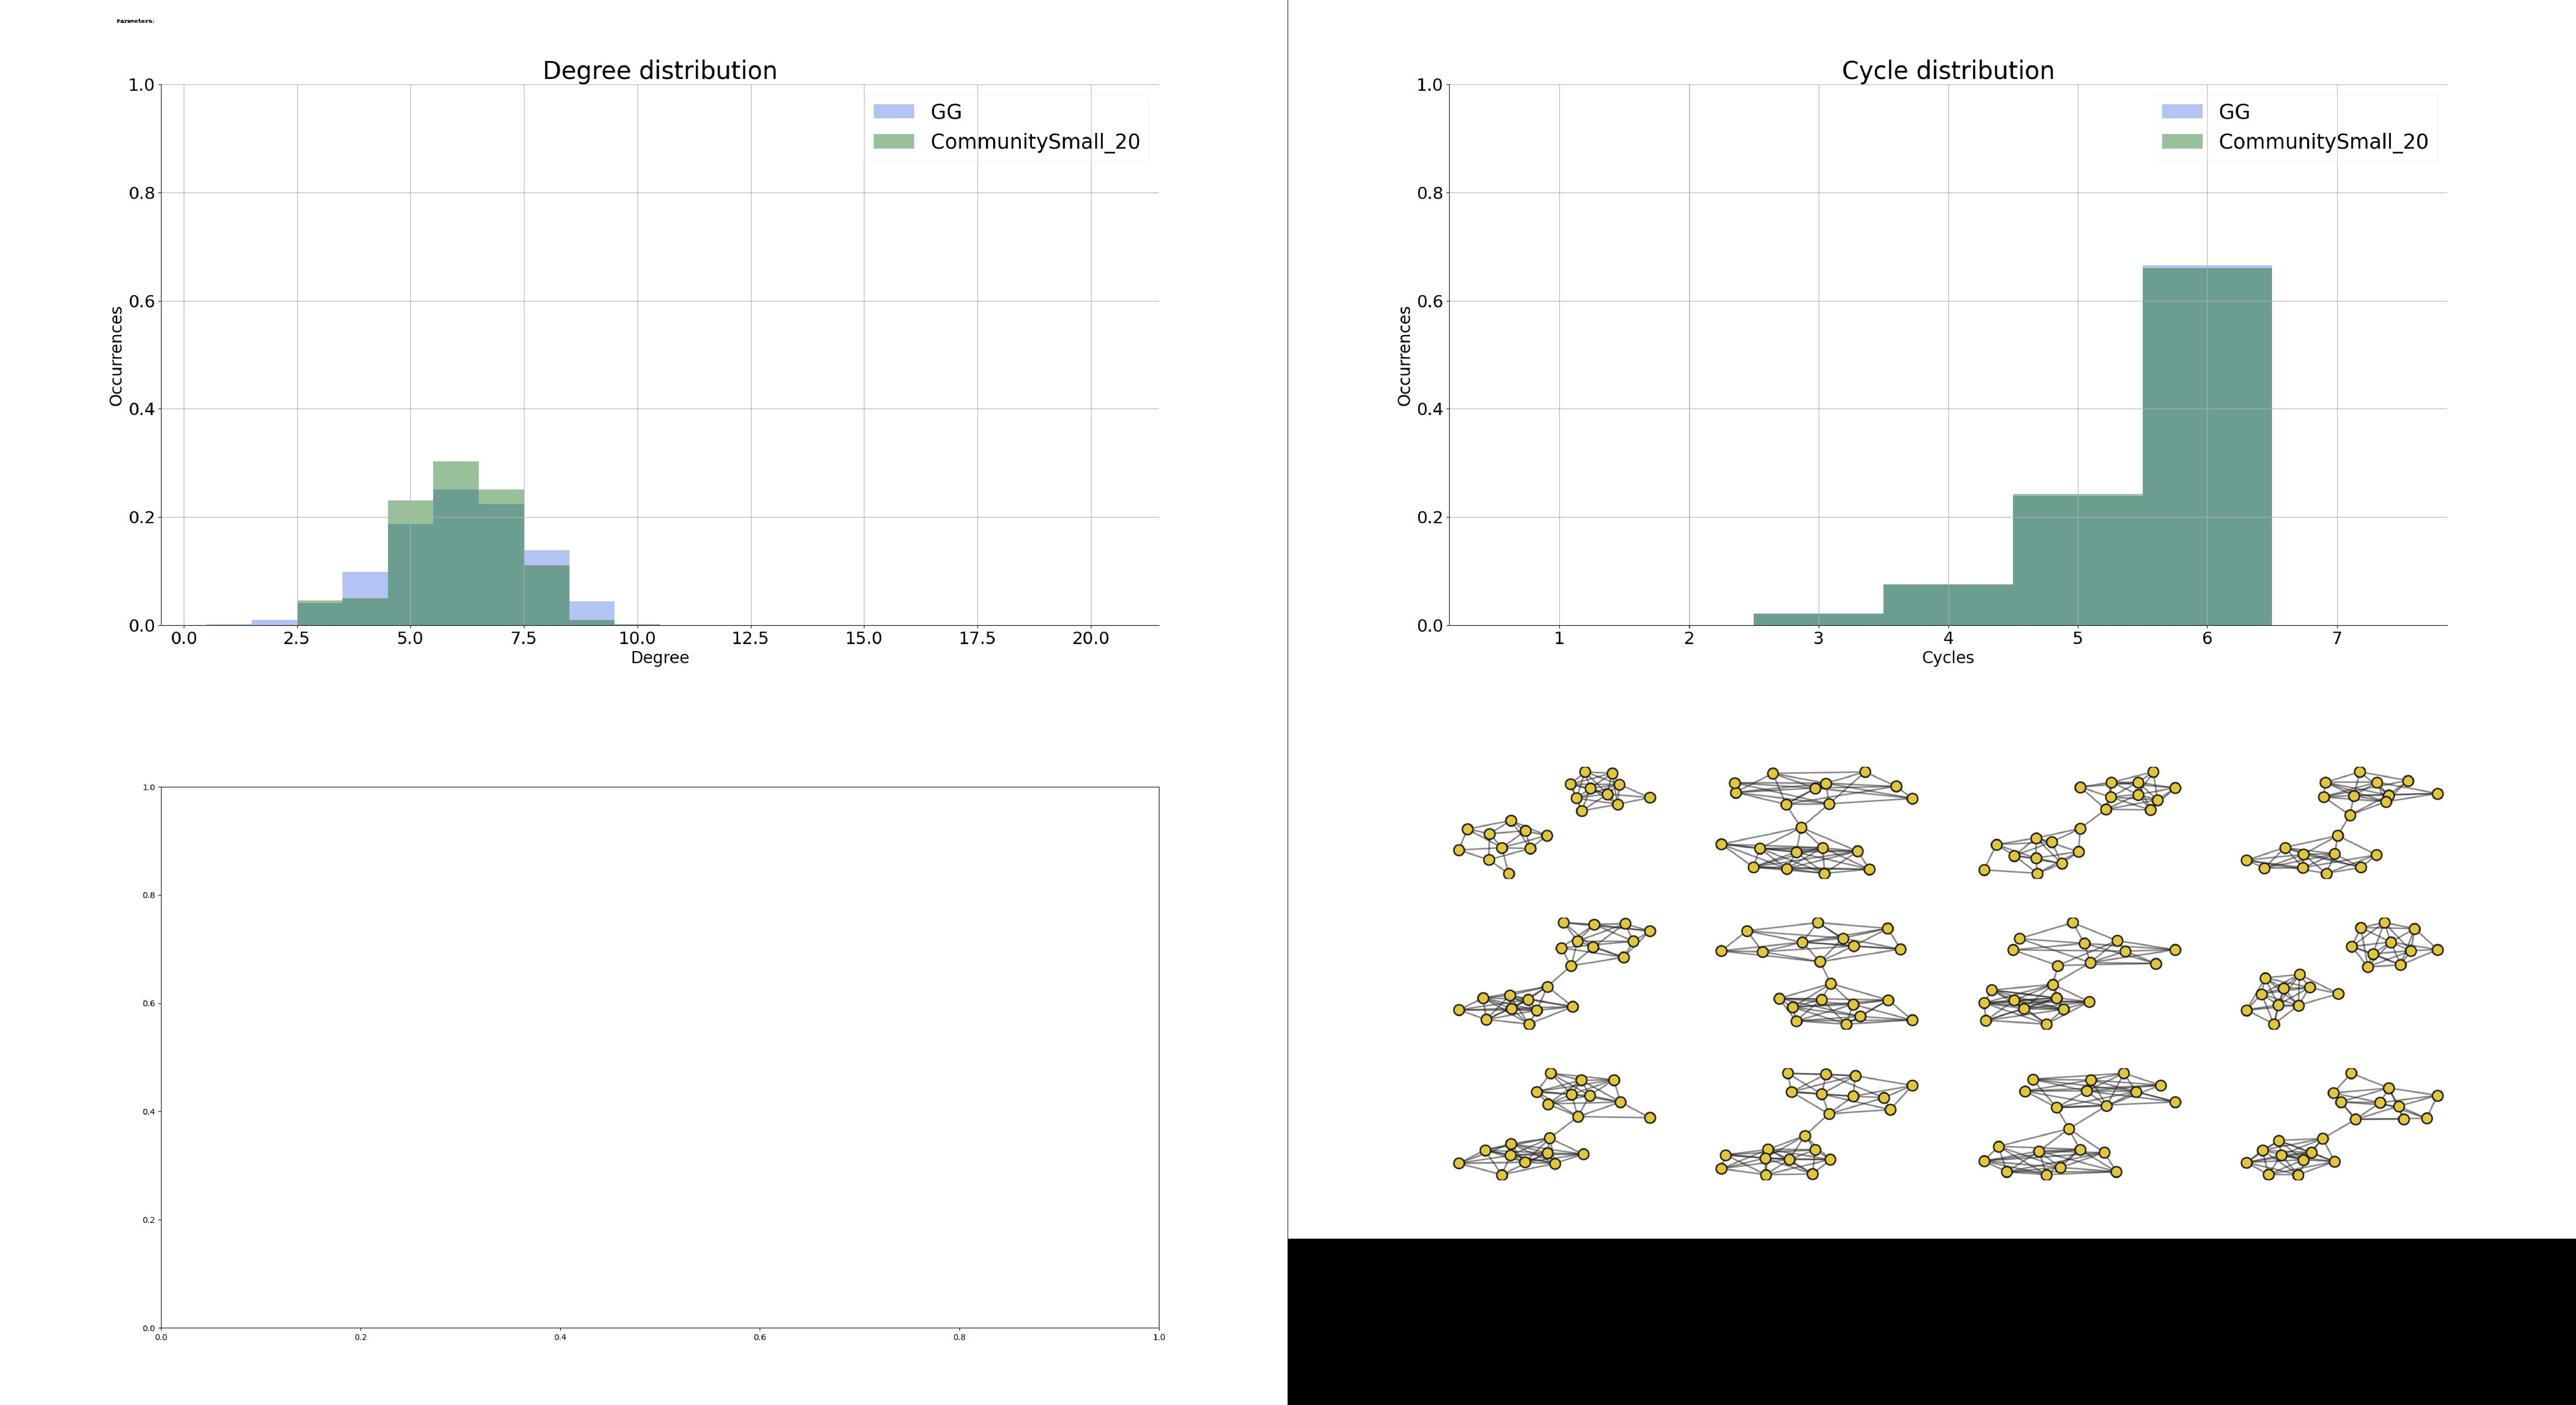
\includegraphics[width=\textwidth]{figures/gggcrp/CommunitySmall_20.pdf}
    \caption[GGG-CRP performance on Community20.]{Community20 performance.}
    \label{fig:community_20}    
    \end{minipage}
    \begin{minipage}{0.475\textwidth}
    \centering
    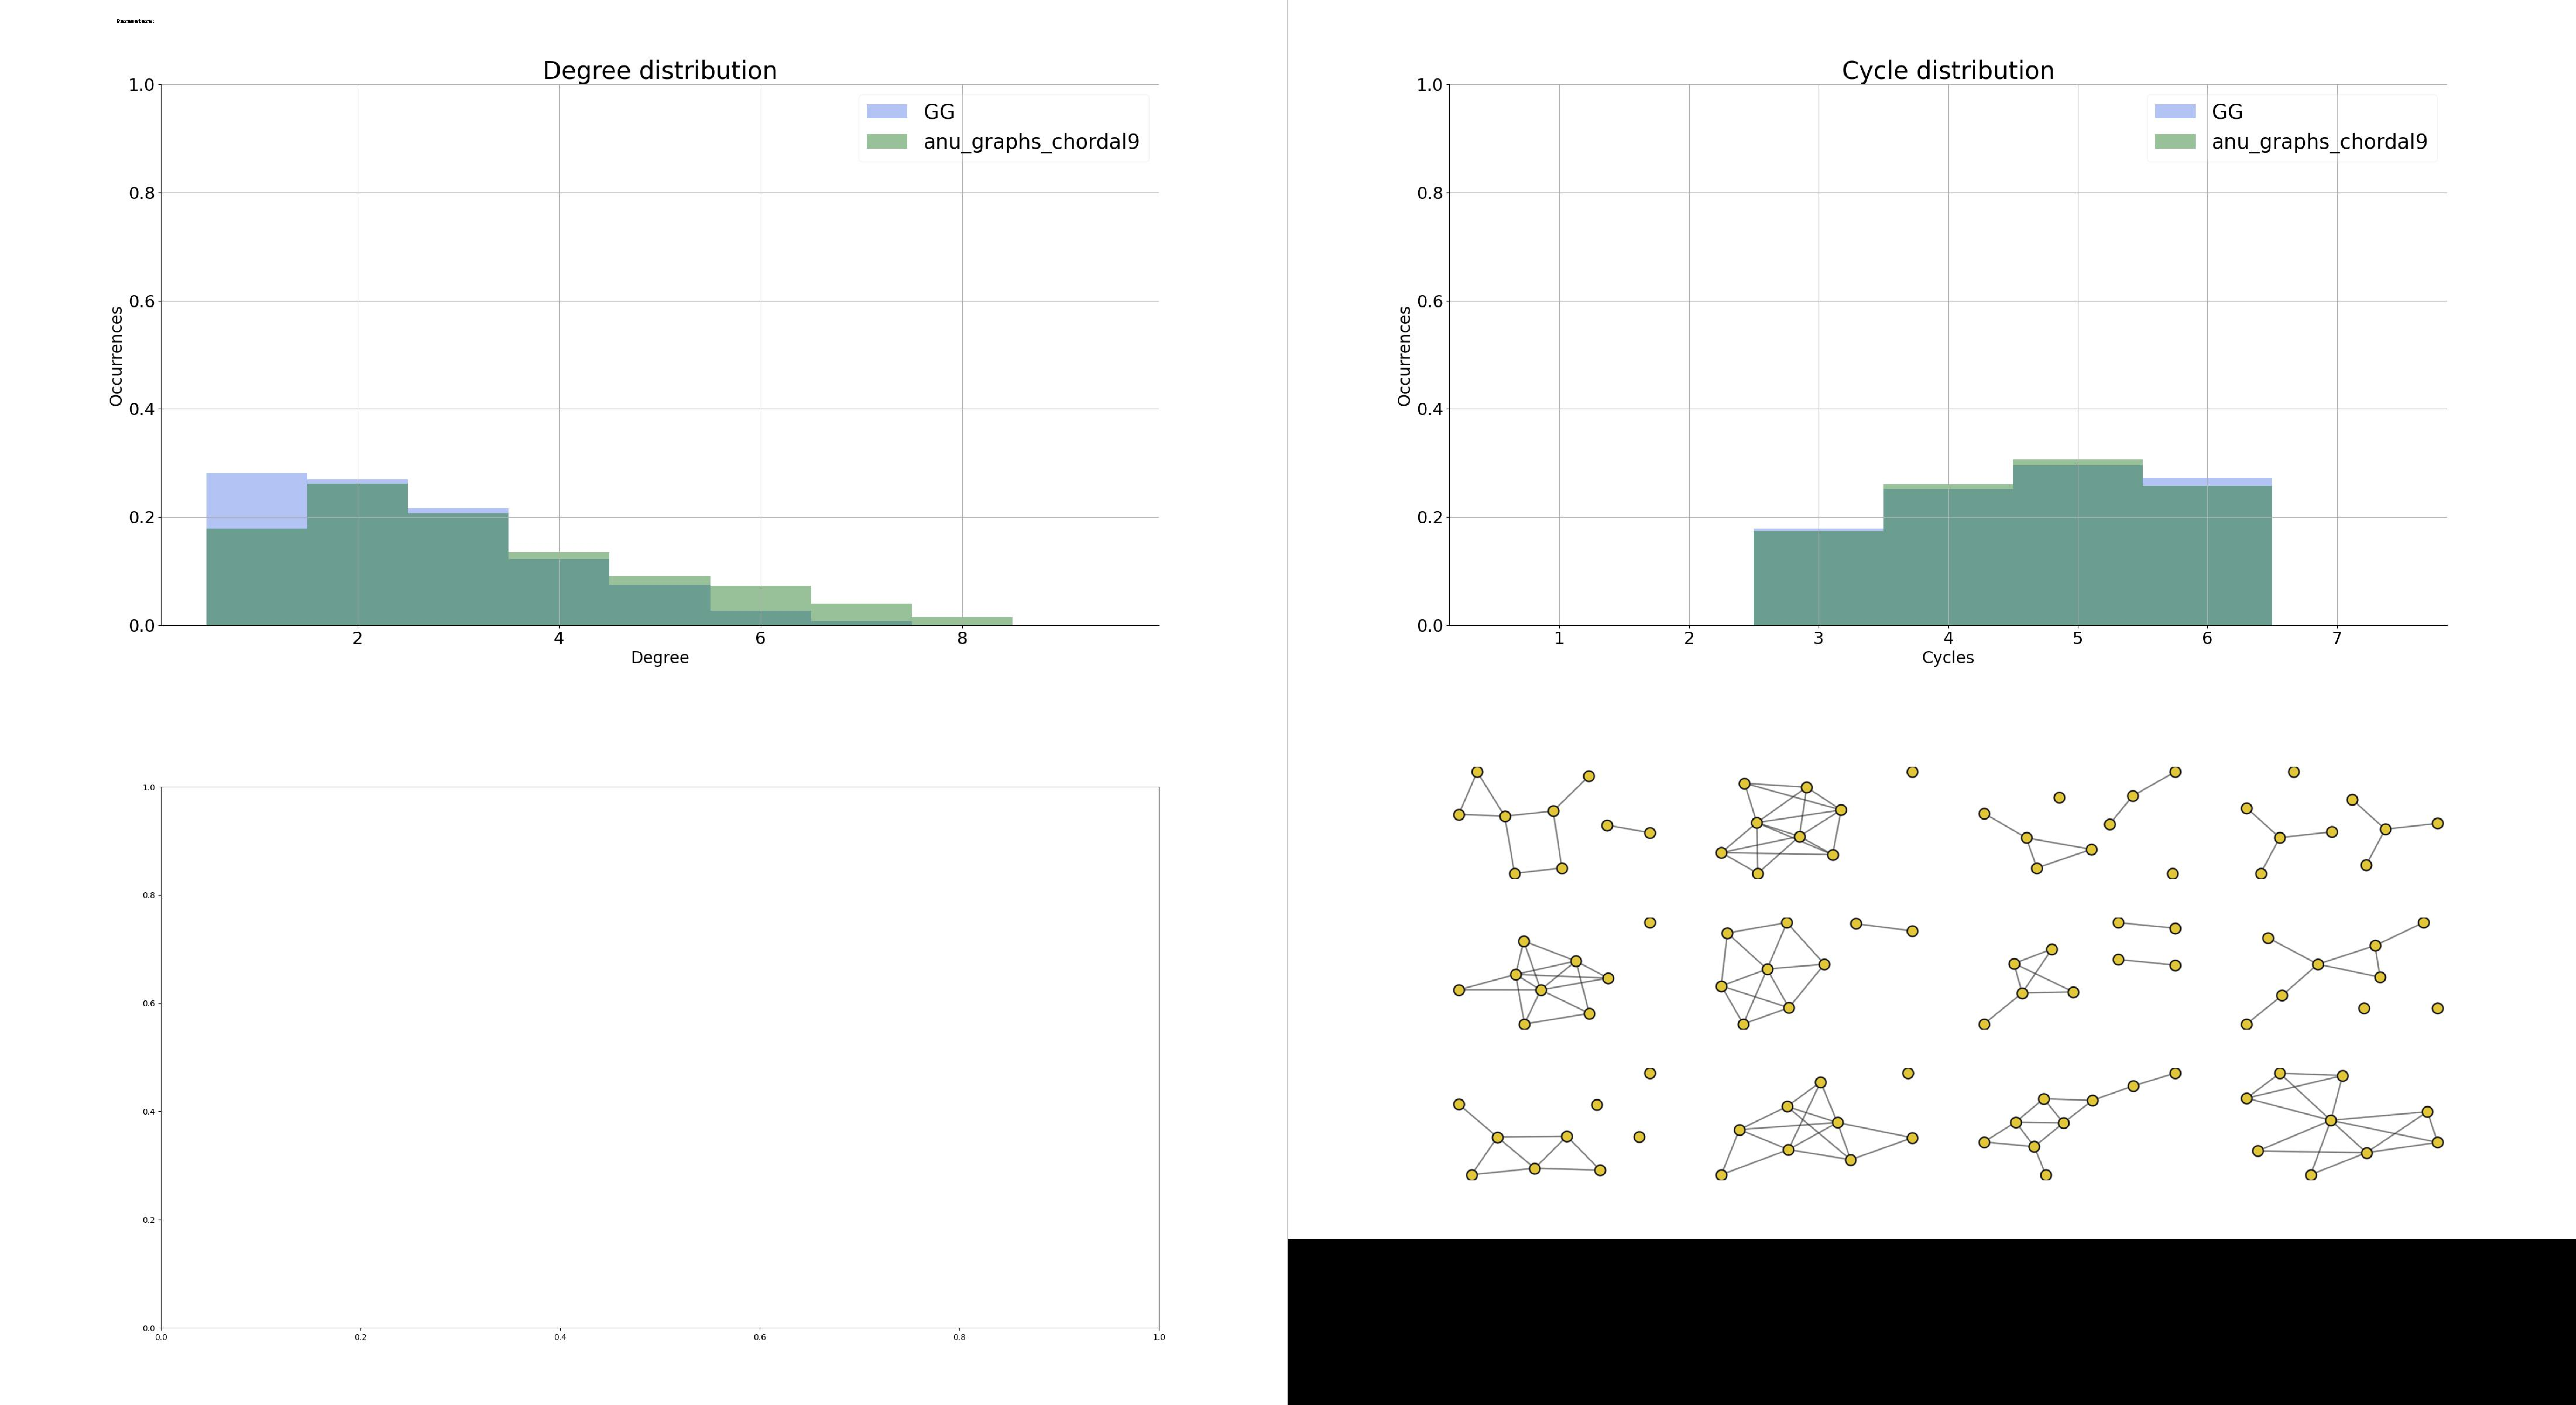
\includegraphics[width=\textwidth]{figures/gggcrp/Chordal9.pdf}
    \caption[GGG-CRP performance on Chordal9.]{Chordal9 performance.}
    \label{fig:chordal9}    
    \end{minipage}
    \hfill
    \begin{minipage}{0.475\textwidth}
    \centering
    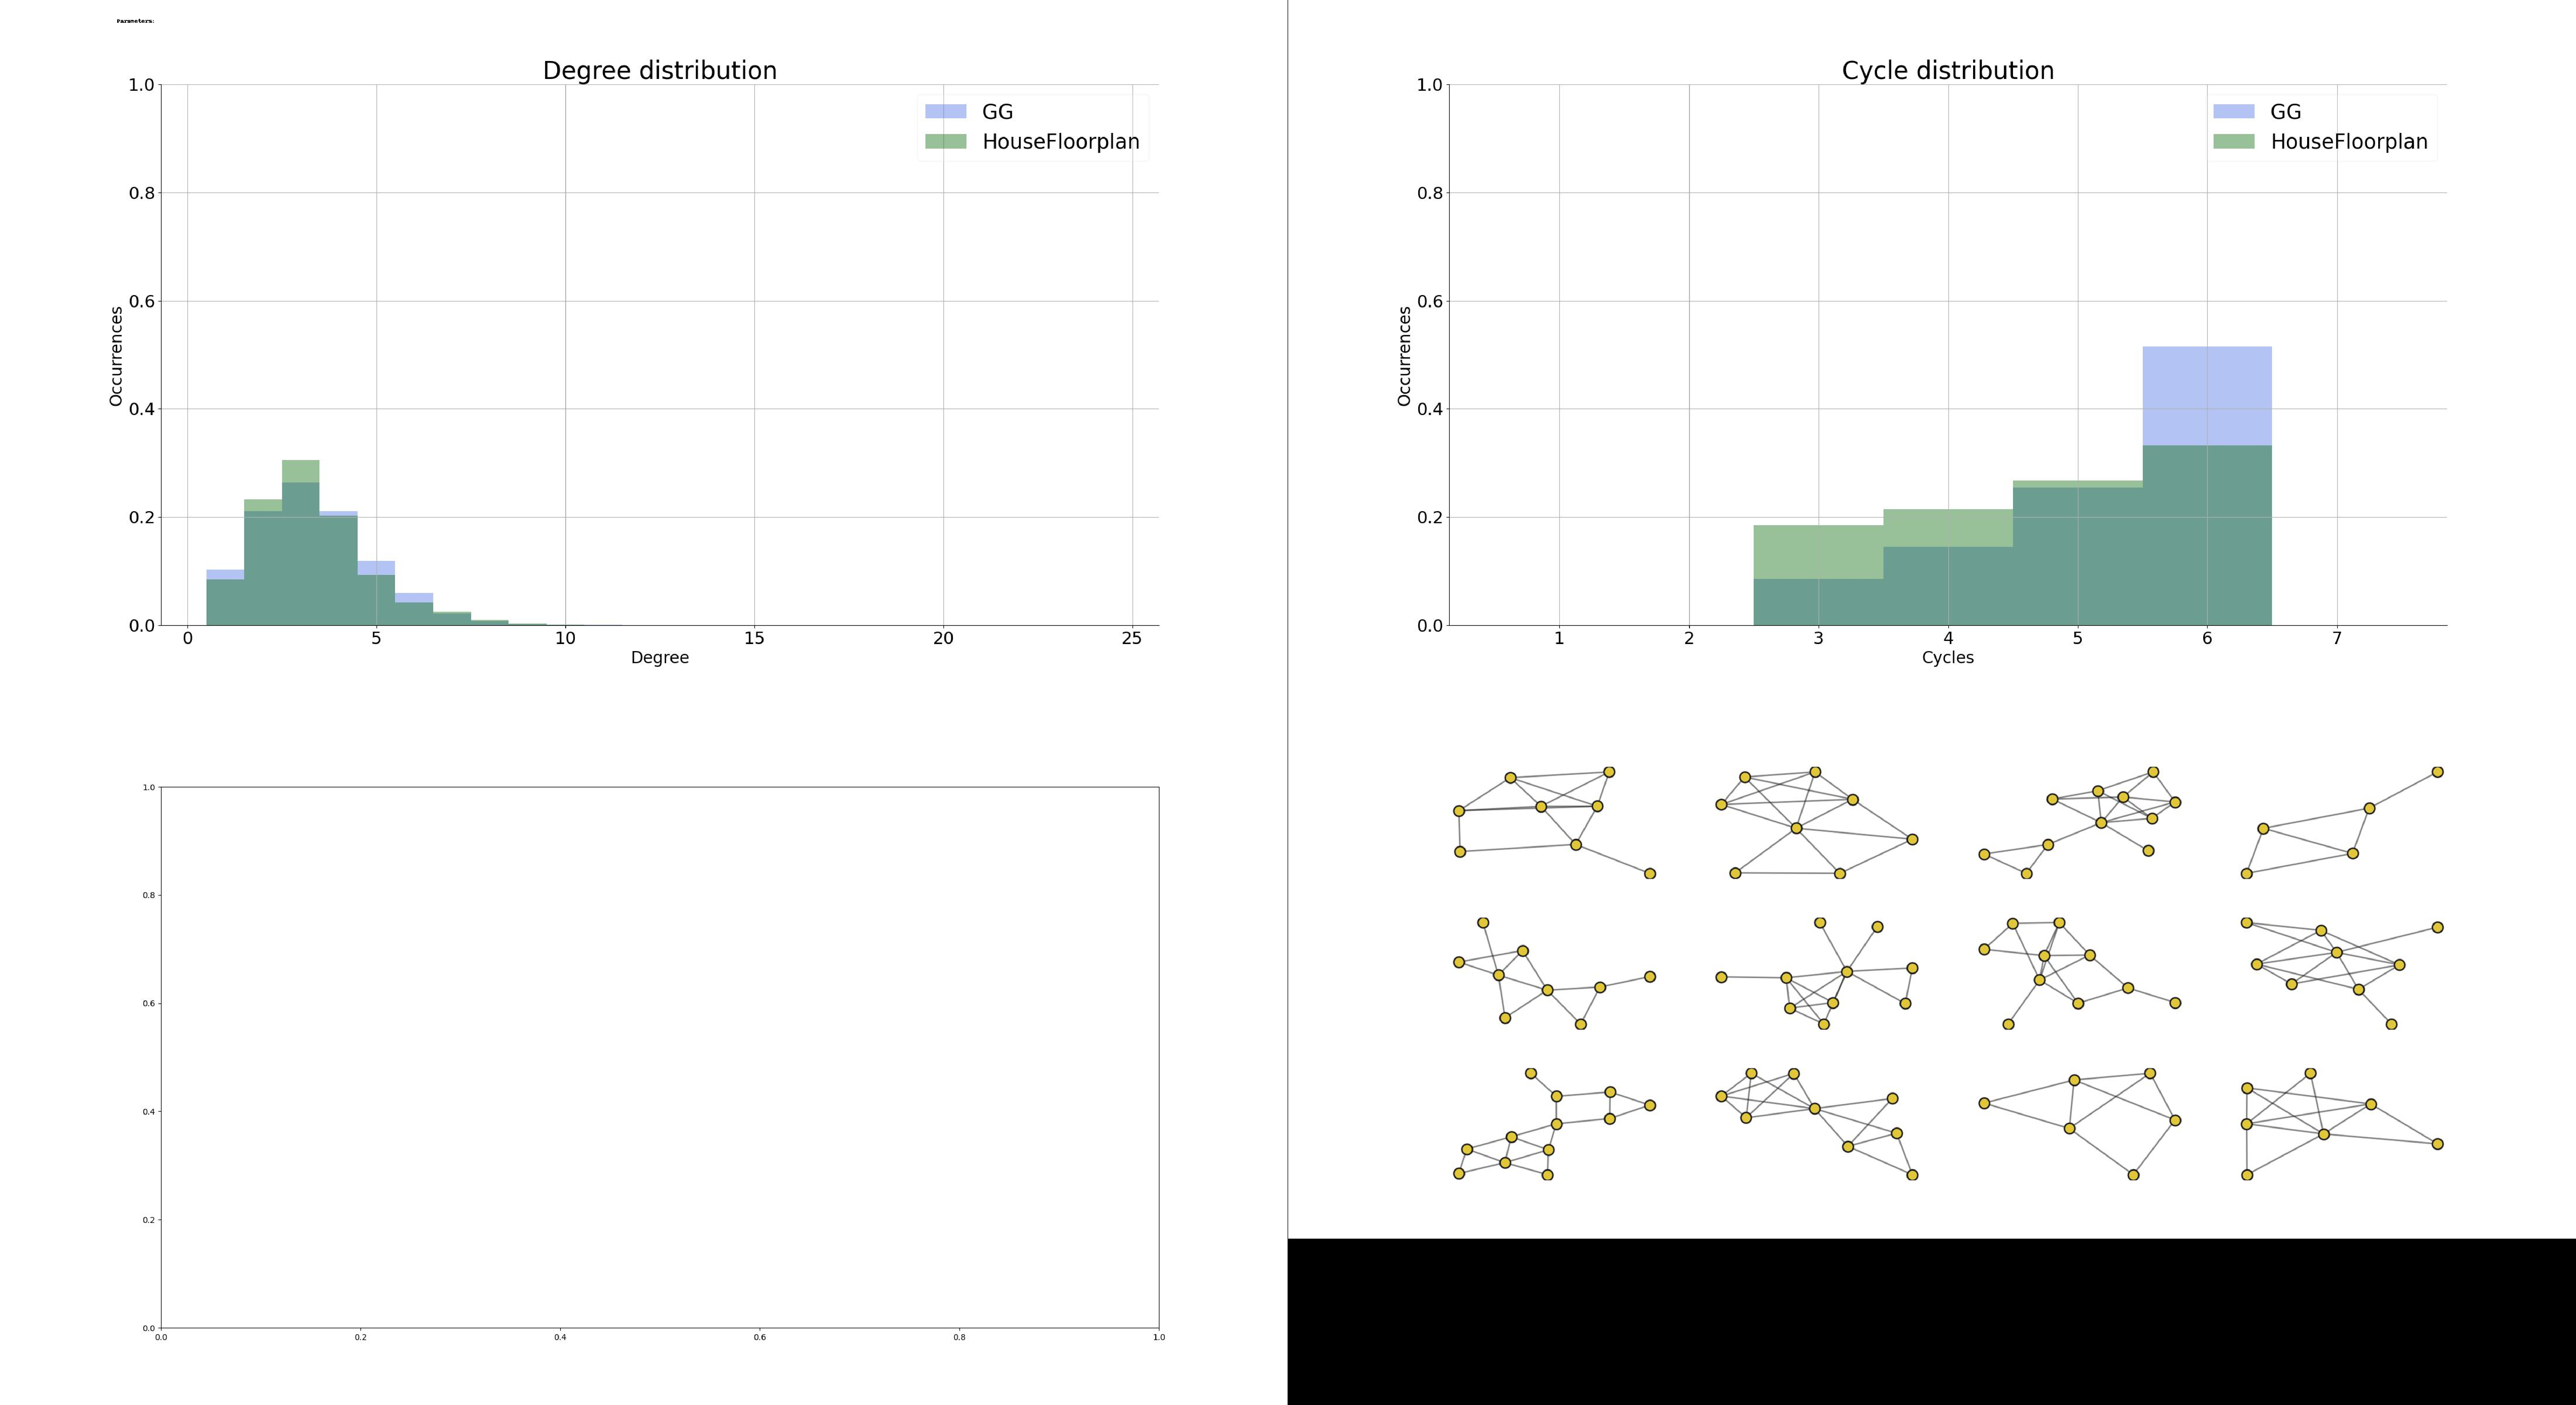
\includegraphics[width=\textwidth]{figures/gggcrp/Housefloorplan.pdf}
    \caption[GGG-CRP performance on HouseFloorplan.]{HouseFloorplan performance.}
    \label{fig:house}    
    \end{minipage}
\end{figure}
Table \ref{tab:novelty} presents the number of isomorphism classes generated by each model during evaluation. Unfortunately, even though it seems that the new approach is consistently better, this comparison would only be valid if GGG-CRP had consistently high expressive power as well, since otherwise, less accurate generators naturally produce graphs not present in the dataset. Nevertheless, we are at least satisfied that GGG-CRP does not suffer from a lack of novelty, which is a common issue for other autoregressive models.
\begin{table}[H]
\centering
\caption[Comparison of novelty and diversity between GG-GAN and GGG-CRP.]{Comparison of novelty and diversity between GG-GAN and GGG-CRP. A higher number of isomorphism classes denotes better performance.}
\label{tab:novelty}
% \setlength{\arrayrulewidth}{0.5mm}
\adjustbox{width=0.6\textwidth}{
\begin{tabular}{lrr}
\toprule
Dataset & GG-GAN & GGG-CRP \\
\midrule
QM9 & 604 & 688 \\
Community20 & 5000 & 5000 \\
Chordal9 & 408 & 2522 \\
HouseFloorplan & \textemdash & 3868 \\
\bottomrule
\end{tabular}
}
\end{table}
We do note another positive behaviour of the GGG-CRP model observed during the training phase: for the Community20 graphs, which possess a very clear community structure, the convergence time compared to the base model was greatly decreased. Less than ten epochs yielded a stable Wasserstein score to obtain the displayed visual results. 

Autoregressive models in general are known to show greater performance when such graph structures are present, and we are pleased that these benefits are also obtained for our model.

\subsection{Summary}
\label{sec:conclusion}

In this section, we presented an approach on how to integrate permutation invariant metrics based on community detection into a Chinese Restaurant Process to perform exchangeable sequence modeling for graph generation. This approach, when integrated into the current best graph GAN model, GG-GAN, yielded a new variation of the model named GGG-CRP. Current results were shown to be comparable to the base model in the wake of strong resource reduction, demonstrating promise. 